\documentclass{article}
\usepackage{tikz,amsmath,siunitx}
\usepackage{pgfplots}
\usepackage{listings}
\usetikzlibrary{arrows,snakes,backgrounds,patterns,matrix,shapes,fit,calc,shadows,plotmarks}
%\usepackage[graphics,tightpage,active]{preview}
%\PreviewEnvironment{tikzpicture}
%\PreviewEnvironment{equation}
%\PreviewEnvironment{equation*}
\title{CS540 Practice Assignment 6}
\author{Dustin Ingram, Aaron Rosenfeld, Tom Wambold}
\newlength{\imagewidth}
\newlength{\imagescale}
\pagestyle{empty}
\thispagestyle{empty}
\lstset{breaklines=true}
\begin{document}
\maketitle
\newpage
\section{Tasks}
\begin{enumerate}
    \item Prove by induction that I tensor A1...At = (I tensor A1)...(I tensor At), or more generally A1...At tensor B1...Bt = (A1 tensor B1)...(At tensor Bt).
    \item Install and test WHT package
    \item Implement recursive and iterative WHT algorithms (in place)
    \item Implement radix 4 recursive and iterative WHT algorithms (in place)
    \item Using the original WHT package, perform timings for recursive and iterative WHT with different sizes of small. Also measure small and compare to iterative. You may want to write a script to generate input to the WHT package measure function.
    \item Using the original WHT package, time random WHTs and produce histogram You will need to write a script to generate and time random WHT algorithms (see the matlab code for a model).
    \item Using the original WHT package, run dynamic programming and compare to recursive, iterative and random. You will need to write a script to perform dynamic programming (see the matlab code for a model).
\end{enumerate}
\newpage
\section{Results}
\subsection{Timings for Iterative vs. Recursive}
  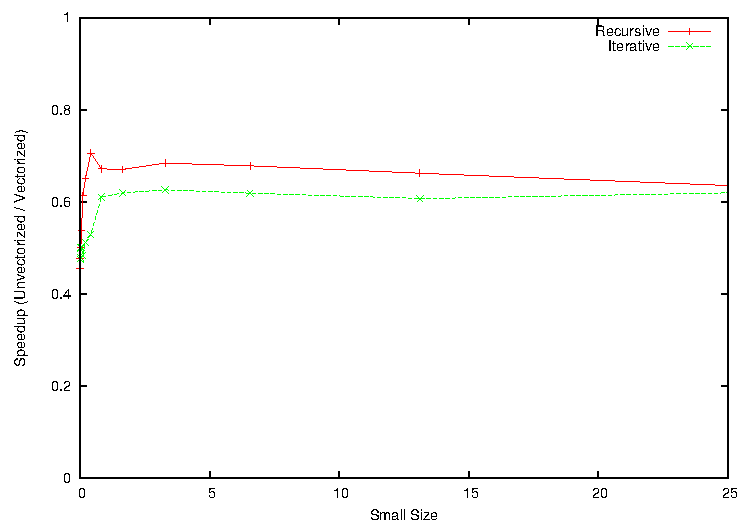
\includegraphics[width=\textwidth]{p6.pdf}
\subsection{Histogram of Timings for Random WHTs}
\begin{center}
\pgfplotsset{width=\textwidth,compat=1.4}
    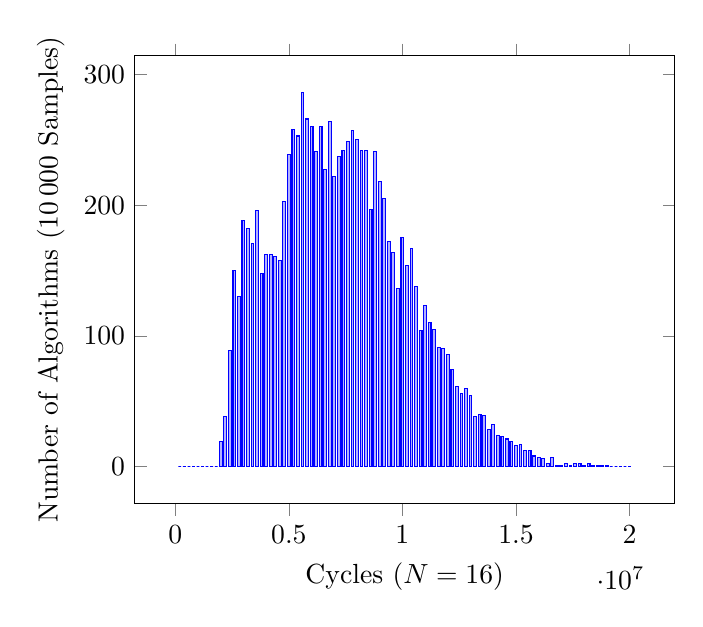
\begin{tikzpicture}
    \begin{axis}[
    ybar,
    bar width=1pt,
    xlabel={Cycles ($N=16$)},
    ylabel=Number of Algorithms (10\,000 Samples),
]
        \addplot coordinates{
(   200000  ,   0   )
(   400000  ,   0   )
(   600000  ,   0   )
(   800000  ,   0   )
(   1000000 ,   0   )
(   1200000 ,   0   )
(   1400000 ,   0   )
(   1600000 ,   0   )
(   1800000 ,   0   )
(   2000000 ,   19  )
(   2200000 ,   38  )
(   2400000 ,   89  )
(   2600000 ,   150 )
(   2800000 ,   130 )
(   3000000 ,   188 )
(   3200000 ,   182 )
(   3400000 ,   171 )
(   3600000 ,   196 )
(   3800000 ,   148 )
(   4000000 ,   162 )
(   4200000 ,   162 )
(   4400000 ,   161 )
(   4600000 ,   158 )
(   4800000 ,   203 )
(   5000000 ,   239 )
(   5200000 ,   258 )
(   5400000 ,   253 )
(   5600000 ,   286 )
(   5800000 ,   266 )
(   6000000 ,   260 )
(   6200000 ,   241 )
(   6400000 ,   260 )
(   6600000 ,   227 )
(   6800000 ,   264 )
(   7000000 ,   222 )
(   7200000 ,   237 )
(   7400000 ,   242 )
(   7600000 ,   249 )
(   7800000 ,   257 )
(   8000000 ,   250 )
(   8200000 ,   242 )
(   8400000 ,   242 )
(   8600000 ,   197 )
(   8800000 ,   241 )
(   9000000 ,   218 )
(   9200000 ,   205 )
(   9400000 ,   172 )
(   9600000 ,   164 )
(   9800000 ,   136 )
(   10000000    ,   175 )
(   10200000    ,   154 )
(   10400000    ,   167 )
(   10600000    ,   138 )
(   10800000    ,   104 )
(   11000000    ,   123 )
(   11200000    ,   110 )
(   11400000    ,   105 )
(   11600000    ,   91  )
(   11800000    ,   90  )
(   12000000    ,   86  )
(   12200000    ,   74  )
(   12400000    ,   61  )
(   12600000    ,   56  )
(   12800000    ,   60  )
(   13000000    ,   54  )
(   13200000    ,   38  )
(   13400000    ,   40  )
(   13600000    ,   39  )
(   13800000    ,   28  )
(   14000000    ,   32  )
(   14200000    ,   24  )
(   14400000    ,   23  )
(   14600000    ,   21  )
(   14800000    ,   19  )
(   15000000    ,   16  )
(   15200000    ,   17  )
(   15400000    ,   12  )
(   15600000    ,   12  )
(   15800000    ,   8   )
(   16000000    ,   7   )
(   16200000    ,   6   )
(   16400000    ,   2   )
(   16600000    ,   7   )
(   16800000    ,   1   )
(   17000000    ,   1   )
(   17200000    ,   2   )
(   17400000    ,   1   )
(   17600000    ,   2   )
(   17800000    ,   2   )
(   18000000    ,   1   )
(   18200000    ,   2   )
(   18400000    ,   1   )
(   18600000    ,   1   )
(   18800000    ,   1   )
(   19000000    ,   1   )
(   19200000    ,   0   )
(   19400000    ,   0   )
(   19600000    ,   0   )
(   19800000    ,   0   )
(   20000000    ,   0   )
};
    \end{axis}
    \end{tikzpicture}
    \end{center}

\subsection{Results of running Dynamic Programming}
{\footnotesize
\begin{tabular}{c l l}
    $N$ & Time ($\mu$s) & Plan \\
    \hline
1 & 354.0 & \texttt{small[1]} \\
2 & 357.0 & \texttt{small[2]} \\
3 & 518.0 & \texttt{small[3]} \\
4 & 604.0 & \texttt{small[4]} \\
5 & 1061.0 & \texttt{small[5]} \\
6 & 1379.0 & \texttt{split[small[3],small[3]]} \\
7 & 2210.0 & \texttt{split[small[4],small[3]]} \\
8 & 3647.0 & \texttt{split[small[4],small[4]]} \\
9 & 8005.0 & \texttt{split[small[3],small[3],small[3]]} \\
10 & 16564.0 & \texttt{split[small[4],small[3],small[3]]} \\
11 & 34021.0 & \texttt{split[small[4],small[4],small[3]]} \\
12 & 70951.0 & \texttt{split[small[4],small[4],small[4]]} \\
13 & 192616.0 & \texttt{split[small[3],small[3],small[3],small[2],small[2]]} \\
14 & 385364.0 & \texttt{split[small[3],small[3],small[3],small[3],small[2]]} \\
15 & 769626.0 & \texttt{split[small[3],small[3],small[3],small[3],small[3]]} \\
16 & 1855763.0 & \texttt{split[small[3],small[3],small[3],small[3],small[2],small[2]]} \\
17 & 3715648.0 & \texttt{split[small[3],small[3],small[3],small[3],small[3],small[2]]} \\
    \end{tabular}
}

\end{document}

